\chapter{主模块设计}
\label{cha:fr}
根据实验要求,实验成果应整合算法子任务模块的有关功能,并需要进行完备的主模块设计。本章将介绍整体设计及其设计原因。

\section{系统框架设计}

实验成果的软件系统整体框架图如下:

\begin{figure}[H]
    \centering
    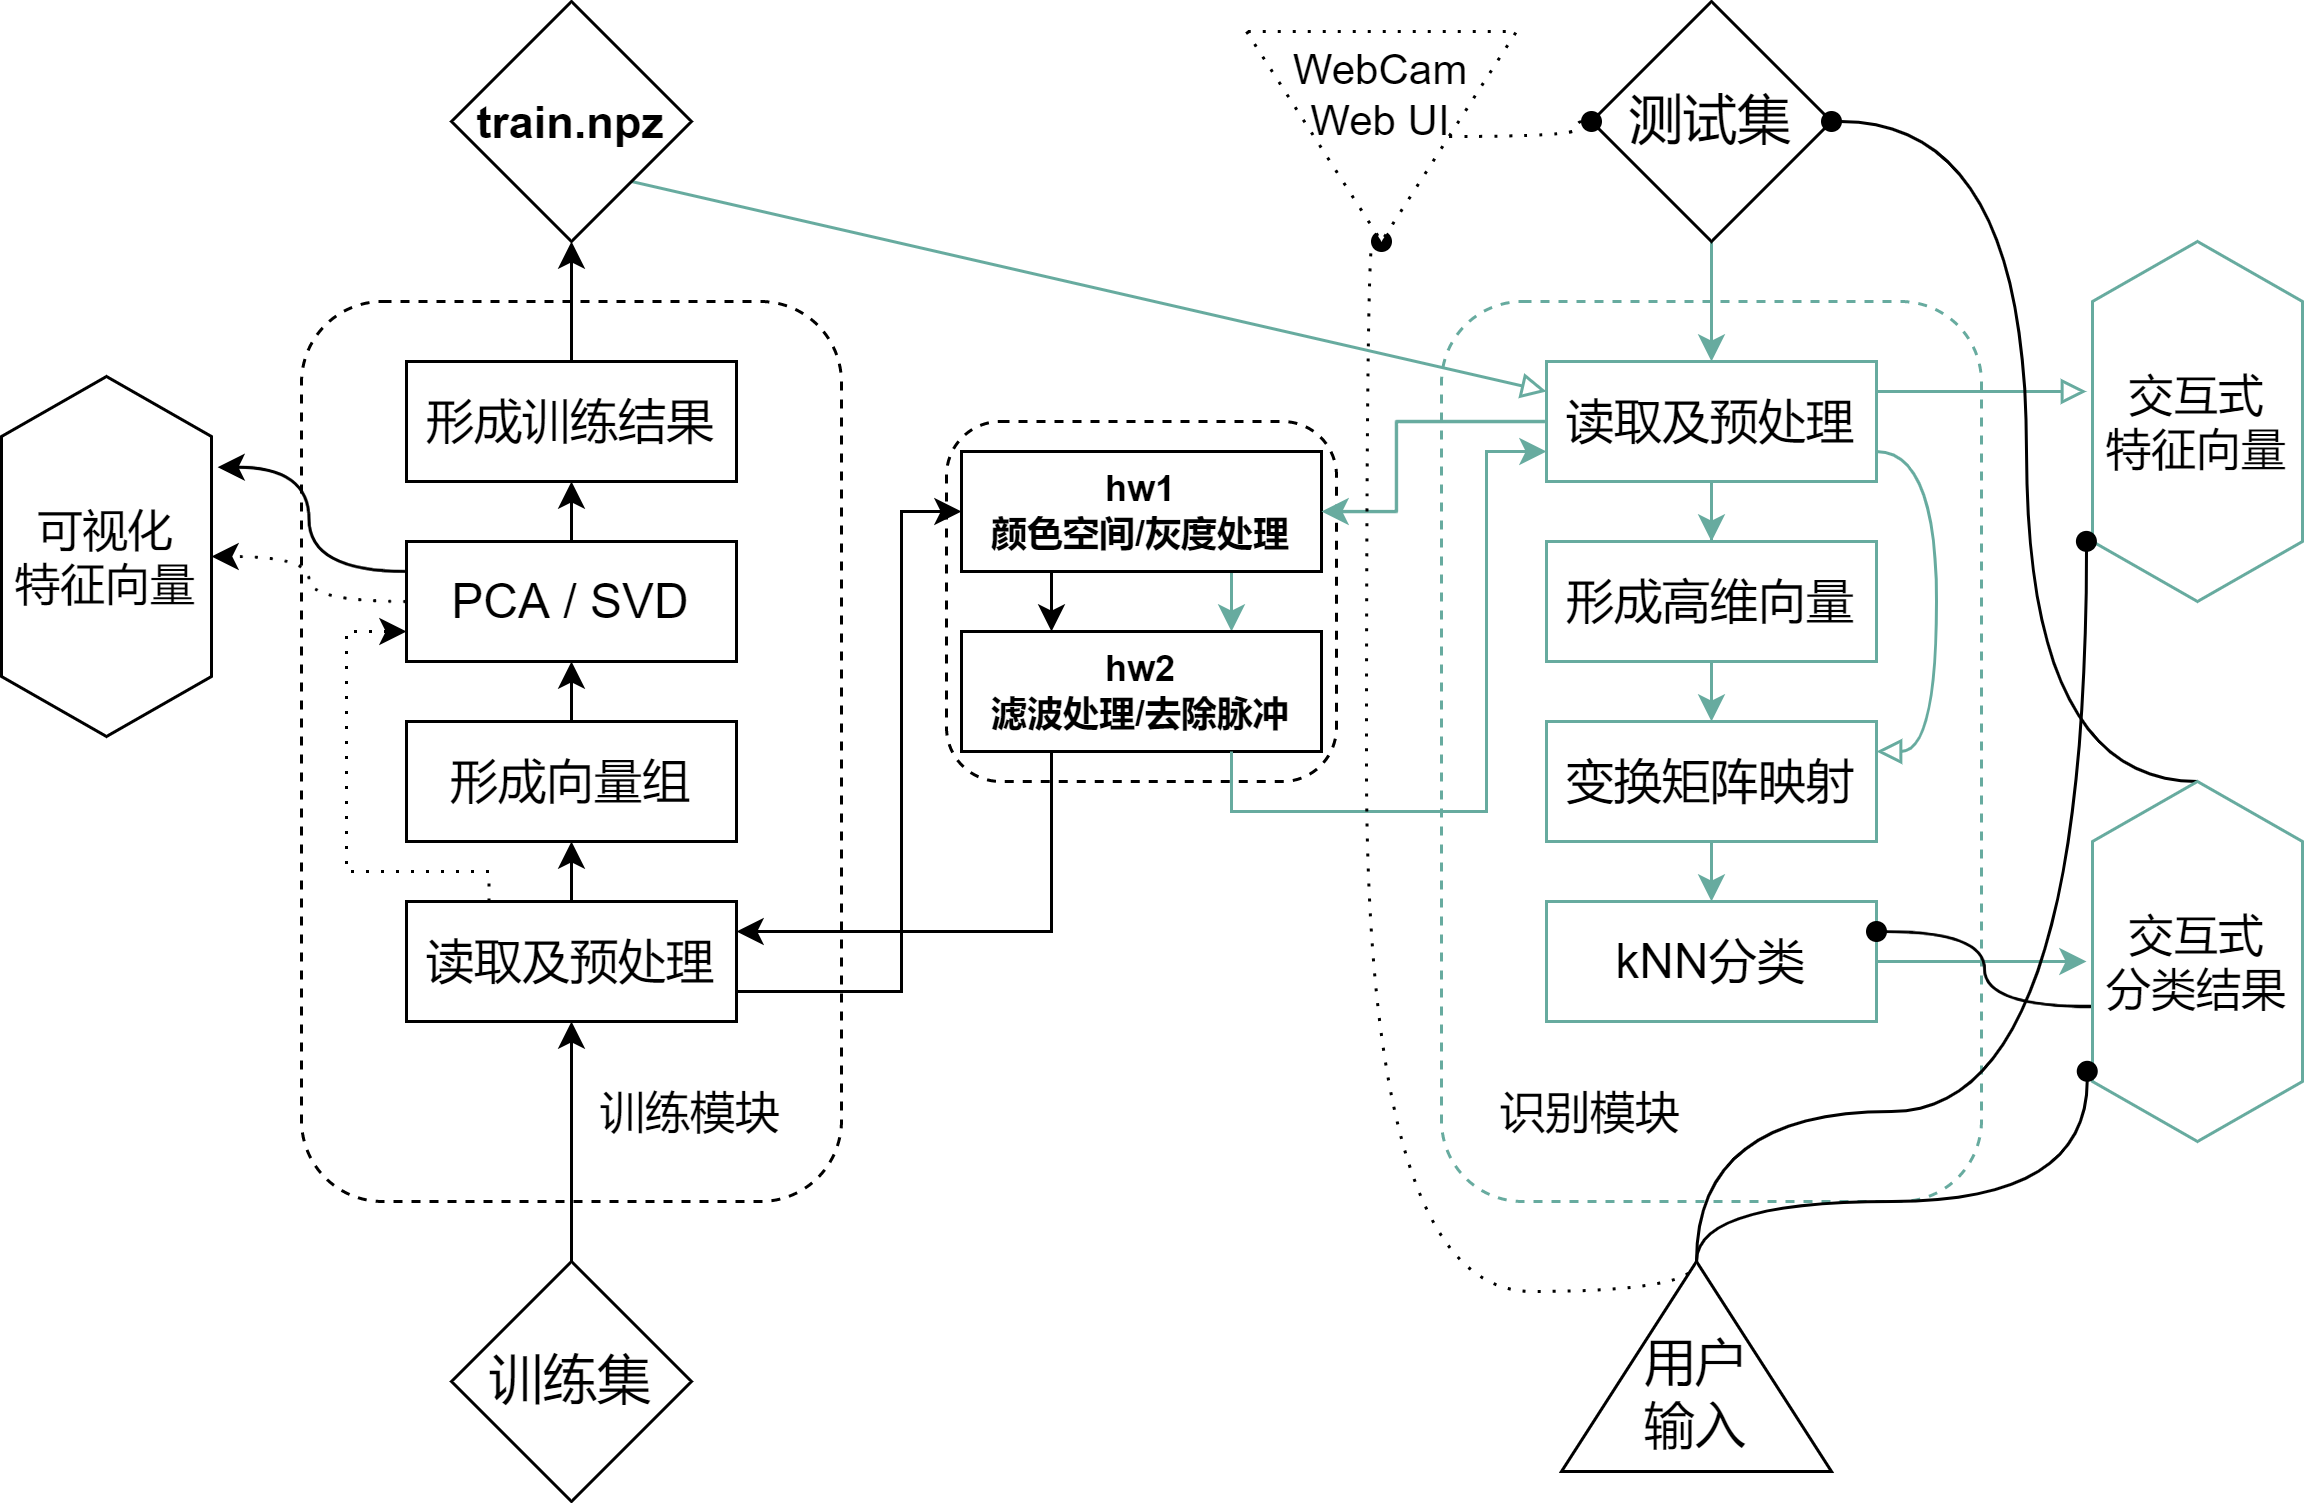
\includegraphics[width=.9\columnwidth]{framework.png}
    \caption{软件框架设计图}
    \label{fig:framework}
\end{figure}

\begin{itemize}
    \item 直接可视化特征向量:对部分单一人脸进行了主成分分析,见\autoref{fig:eig_single}。
    \item WebUI:本软件预留了网页端的相关接口。
\end{itemize}

\subsection{训练集和测试集}
\label{sec:dataset}

数据集均为\verb|600x400|的有露出人脸照片,格式为\verb|.jpg|,有两组样本具有加入噪声后的白边,有一组样本照片部分经过了一次逆时针旋转。约9成的照片加入了随机生成的彩色椒盐噪声。
\begin{itemize}
    \item 在空域中,椒盐噪声分别指极暗或极亮的像素点,且明显不属于原照片的内容,其又名脉冲噪声。
    \item 此处的彩色噪声,指任意单通道的值极大或极小。
\end{itemize}

\begin{figure}[H]
	\begin{minipage}{0.45\textwidth}
		\centering
		
\includegraphics[width=.75\columnwidth]{s26_7.jpg}
		\caption{含椒盐噪声。本组样本的照片,含戴上眼镜与未带眼镜两种。}
	\end{minipage}\hfill
	\begin{minipage}{0.45\textwidth}
		\centering
		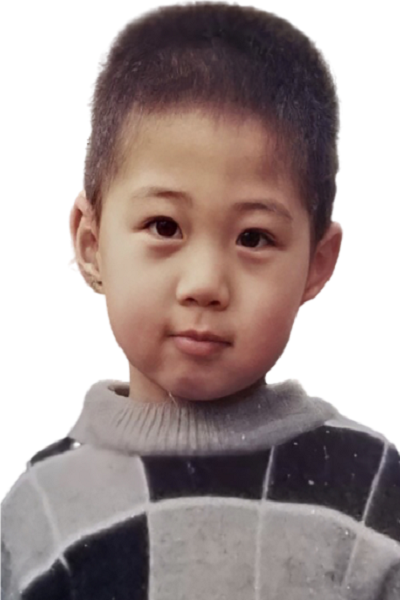
\includegraphics[width=.75\columnwidth]{s13_9.jpg}
		\caption{不含椒盐噪声。本组样本的照片,含不同年龄形态。}
	\end{minipage}
\end{figure}

\section{用户交互框架设计}
\label{sec:ui}

本软件共有两个交互窗口,等待用户输入,见\autoref{fig:ui}。

\begin{figure}[H]
    \centering
    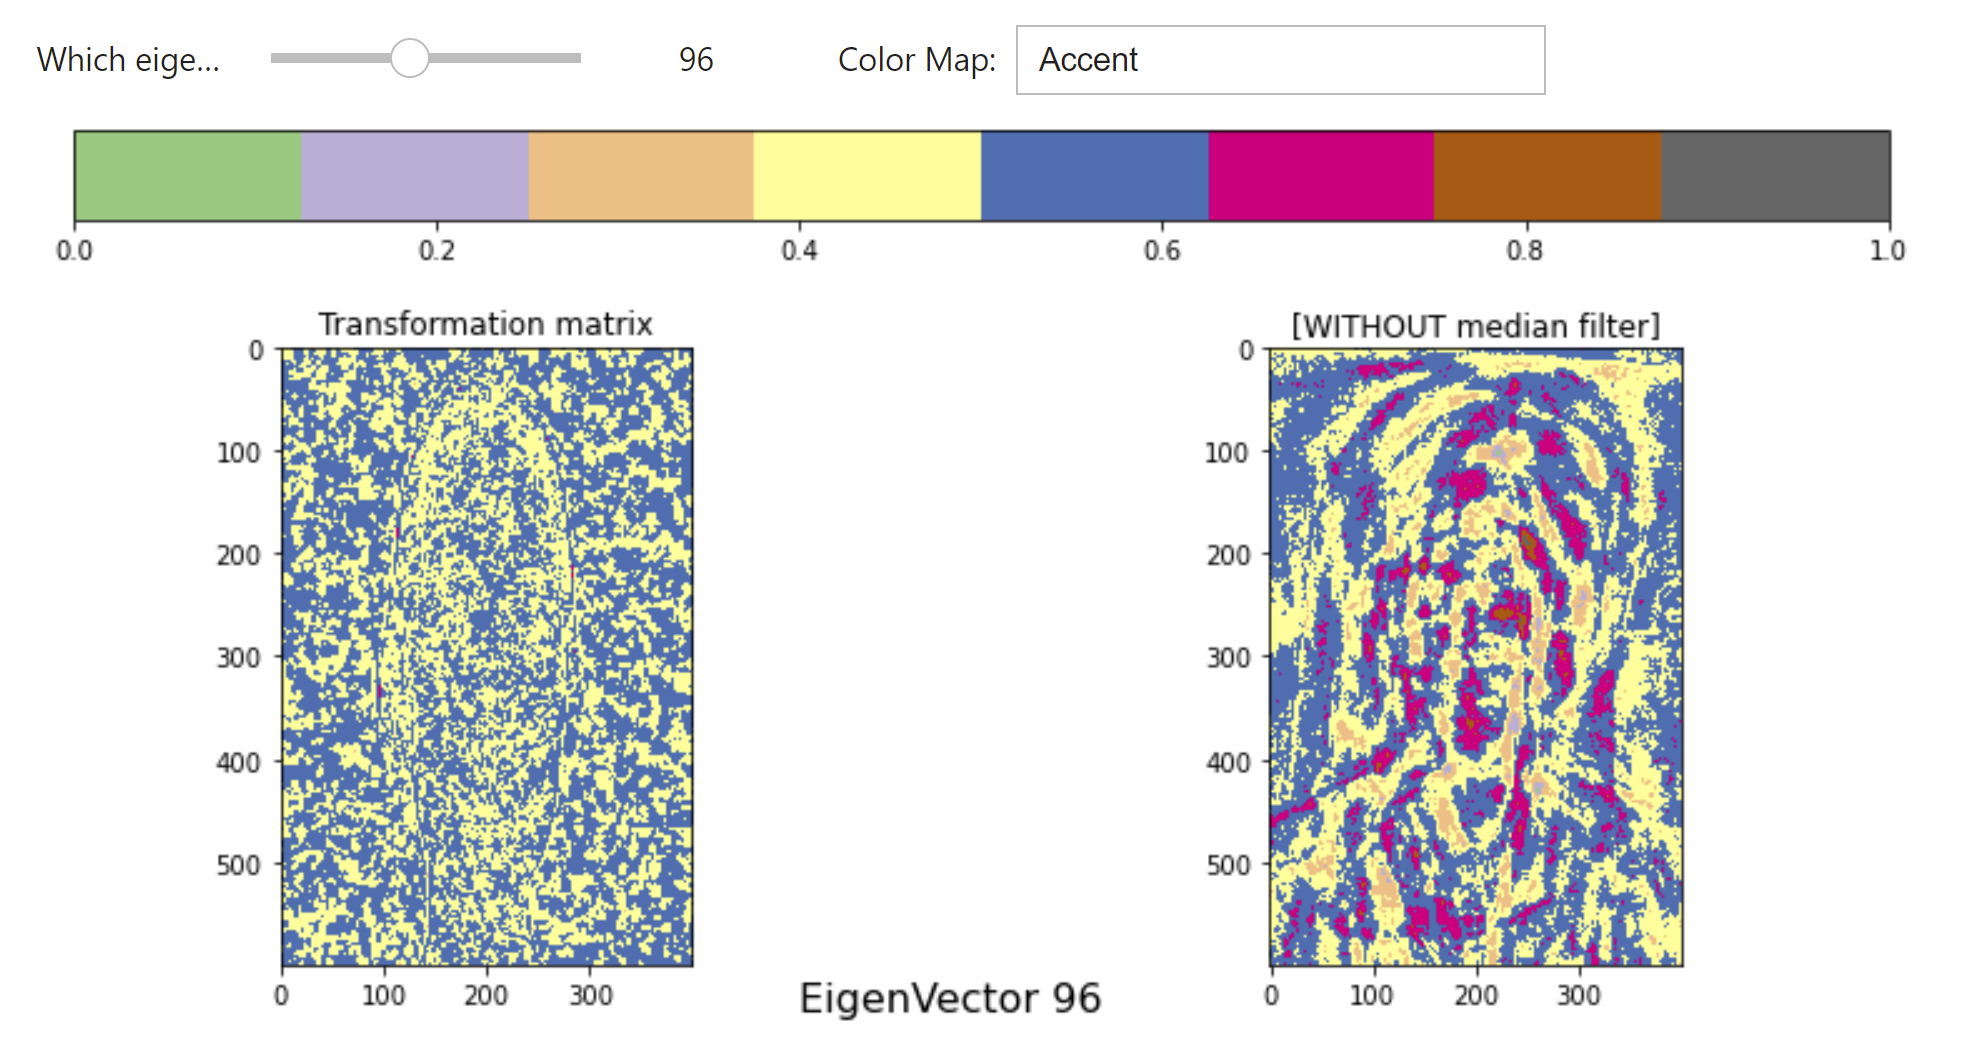
\includegraphics[width=.6\columnwidth]{ui1}
    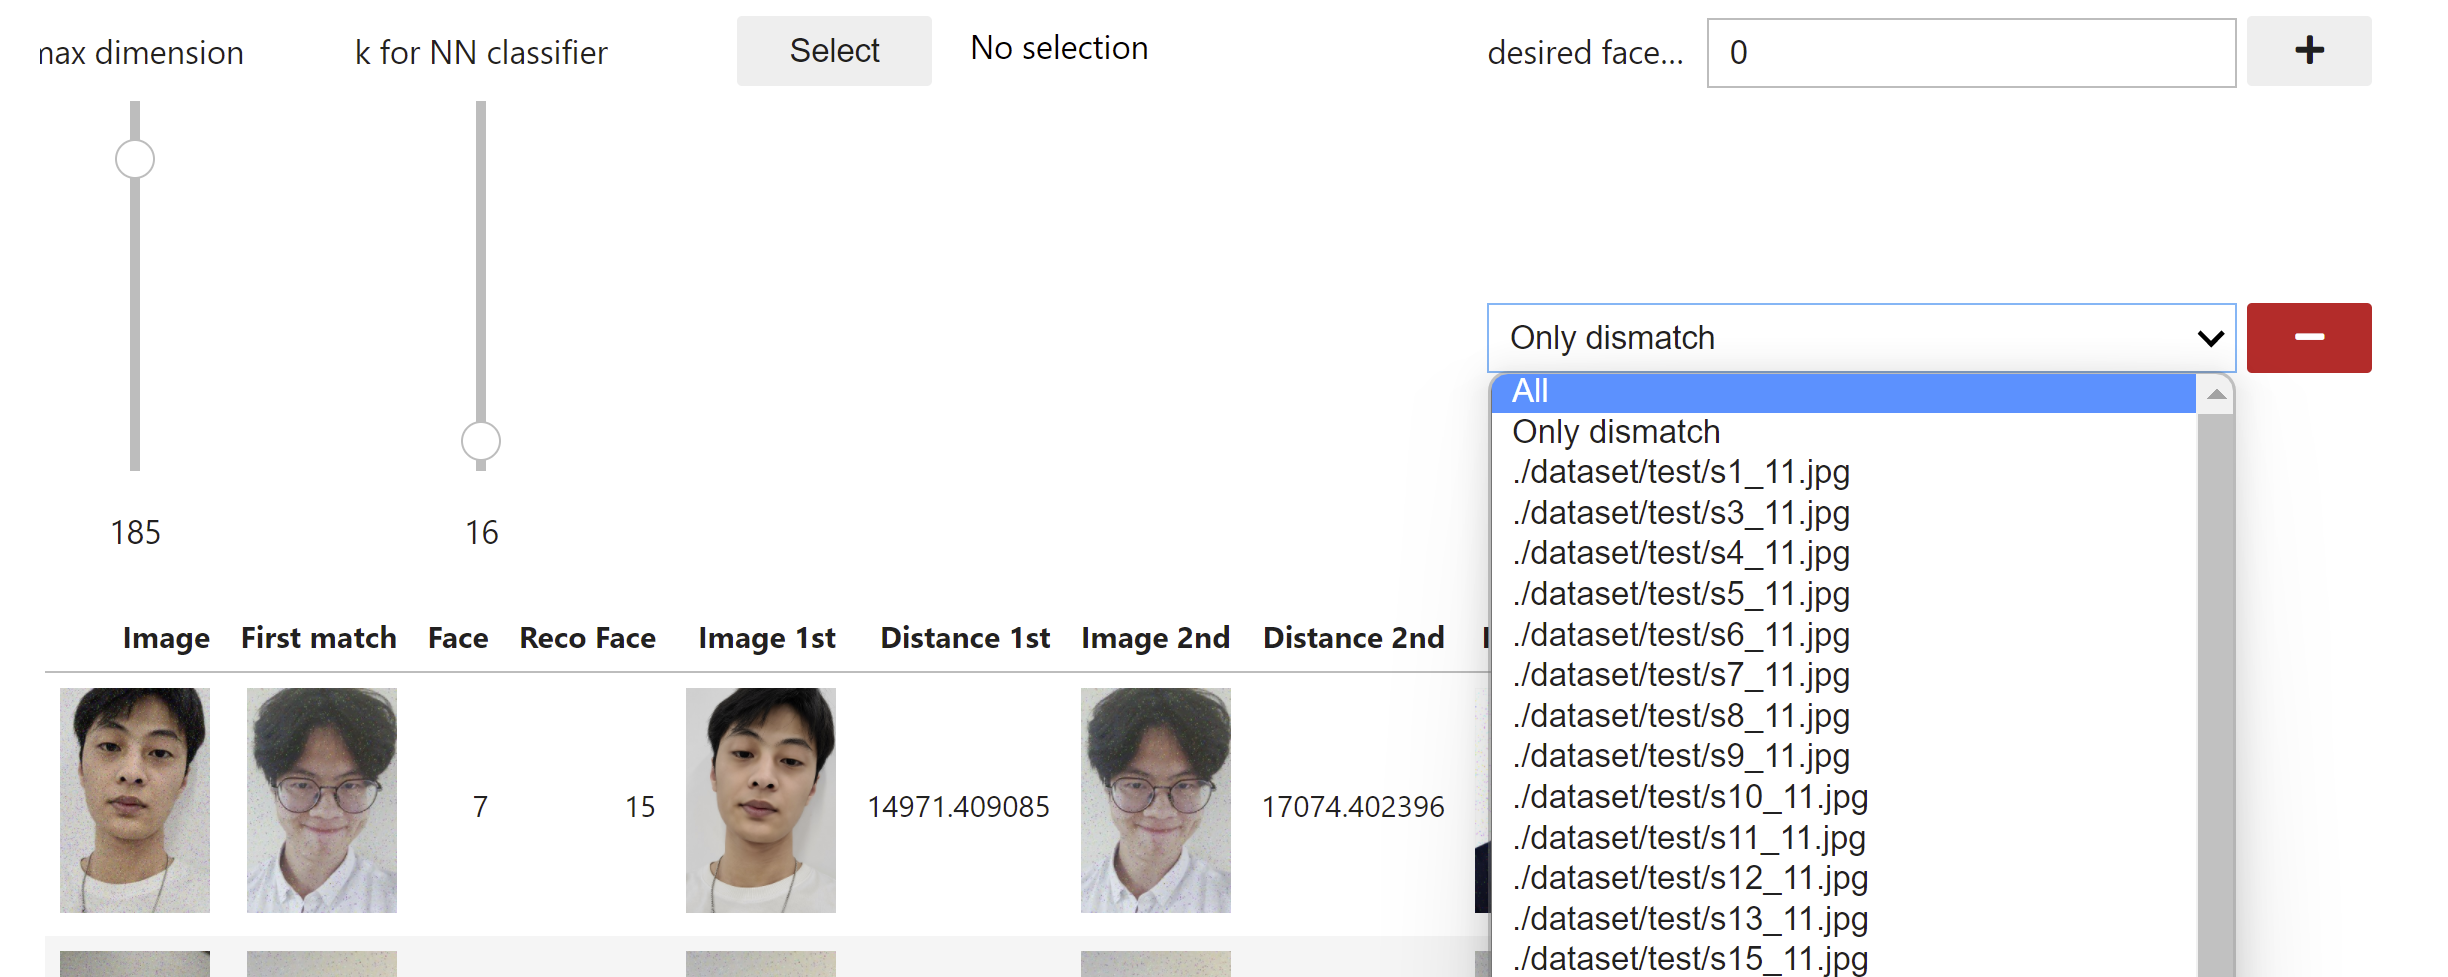
\includegraphics[width=.6\columnwidth]{ui2}
    \caption{第一个交互窗口展示特征向量重新投影至二维空间的情形,第二个交互窗口展示了分类的具体情况。}
    \label{fig:ui}
\end{figure}

第一个交互窗口允许用户选择一种matplotlib中定义了的颜色空间展示图像结果。根据\autoref{sec:eig}的结果,合适的颜色空间可让人眼更易于发现特定的数据区别。默认值无特定含义。

第二个交互窗口是一个动态加载的文件列表,默认加载所有测试集图片。在下拉框内可选择查看所有已加载文件,或是仅列出与样本标记不匹配的识别结果,抑或是选择单个文件。选择单个文件的环境下,用户可点击减号将该文件移出文件列表,也可以在上方选择文件后,给予相应的人脸标记,加入文件列表。配合对参数$k, d$的修改,本界面对系列识别结果有着直观的展示,同时非常适合用户调参和问题分析。

\section{开发工具选择}
\label{sec:dev}
本实验的基本要求是撰写Matlab源代码(\verb|.m|),并在算法实现的基础上完成一个可供用户使用的GUI界面。鉴于:1.在Python环境下numpy、pandas、scipy、matplotlib等宏包,对于Matlab在矩阵计算等方面的功能有较好的互补性和支持(\autoref{listing:dev});2.这些宏包配合ipython kernel与jupyter在开发及展示、移植上相较于Matlab更为方便;3.使用Python环境可以运用numba等工具,加速在中值滤波(\autoref{sec:median-filter0})等处使用到的循环流程,避免实现验证时的长时间等待,便于接轨实际应用。{\bfseries 因此,本实验的算法代码将以笔记本(\verb|.ipynb|)和Python源文件(\verb|.py|)的方式提供。}

同时,本节将对本次实验所用到的开发工具作简单的介绍,并重点分析其优势和它们之间的关系。使用方法此处不再赘述。

\begin{itemize}
\item 本实验代码的算法实现部分,大部分可经批量修改后由Matlab直接使用。例如以下两份节选代码,可实现对矩阵的相同操作。此处内置函数的实现方法(如\verb|eig|),在两种环境内也一般是使用LAPACK库。\cite{Tobler_2019, Numpy_eig}
\begin{listing}[!ht]
% https://www.overleaf.com/learn/latex/Code_Highlighting_with_minted
\begin{minted}[linenos, breaklines, tabsize=2, fontsize=\footnotesize]{matlab}
  [eigValue, eigPreVector] = eig(matMean .* matMean.T) % already sorted
  eigVector = (matMean.T .* eigPreVector) / eigValue
  eigNormalizedVector = eigVector / norm(eigVector, 0)
\end{minted}
\begin{minted}[linenos, breaklines, tabsize=2, fontsize=\footnotesize]{python}
  import numpy as np
  eigValue, eigPreVector = np.linalg.eig(np.dot(matMean, matMean.T)) # already sorted & normalized by eig function
  eigVector = np.dot(matMean.T, eigPreVector) / eigValue
  eigNormalizedVector = eigVector / npMat.norm(eigVector, axis = 0)
\end{minted}
\caption{对矩阵特征向量作转换后(\autoref{sec:pca0}),进行归一化处理(Matlab 和 Python 版本)}
\label{listing:dev}
\end{listing}

\item 使用\textbf{jupyter笔记本},可实现与Matlab相仿的代码、注释书写环境,并对生成数据进行实时终端处理,或是使用数据查看器进行进一步操作。
\begin{figure}[h]
    \centering
    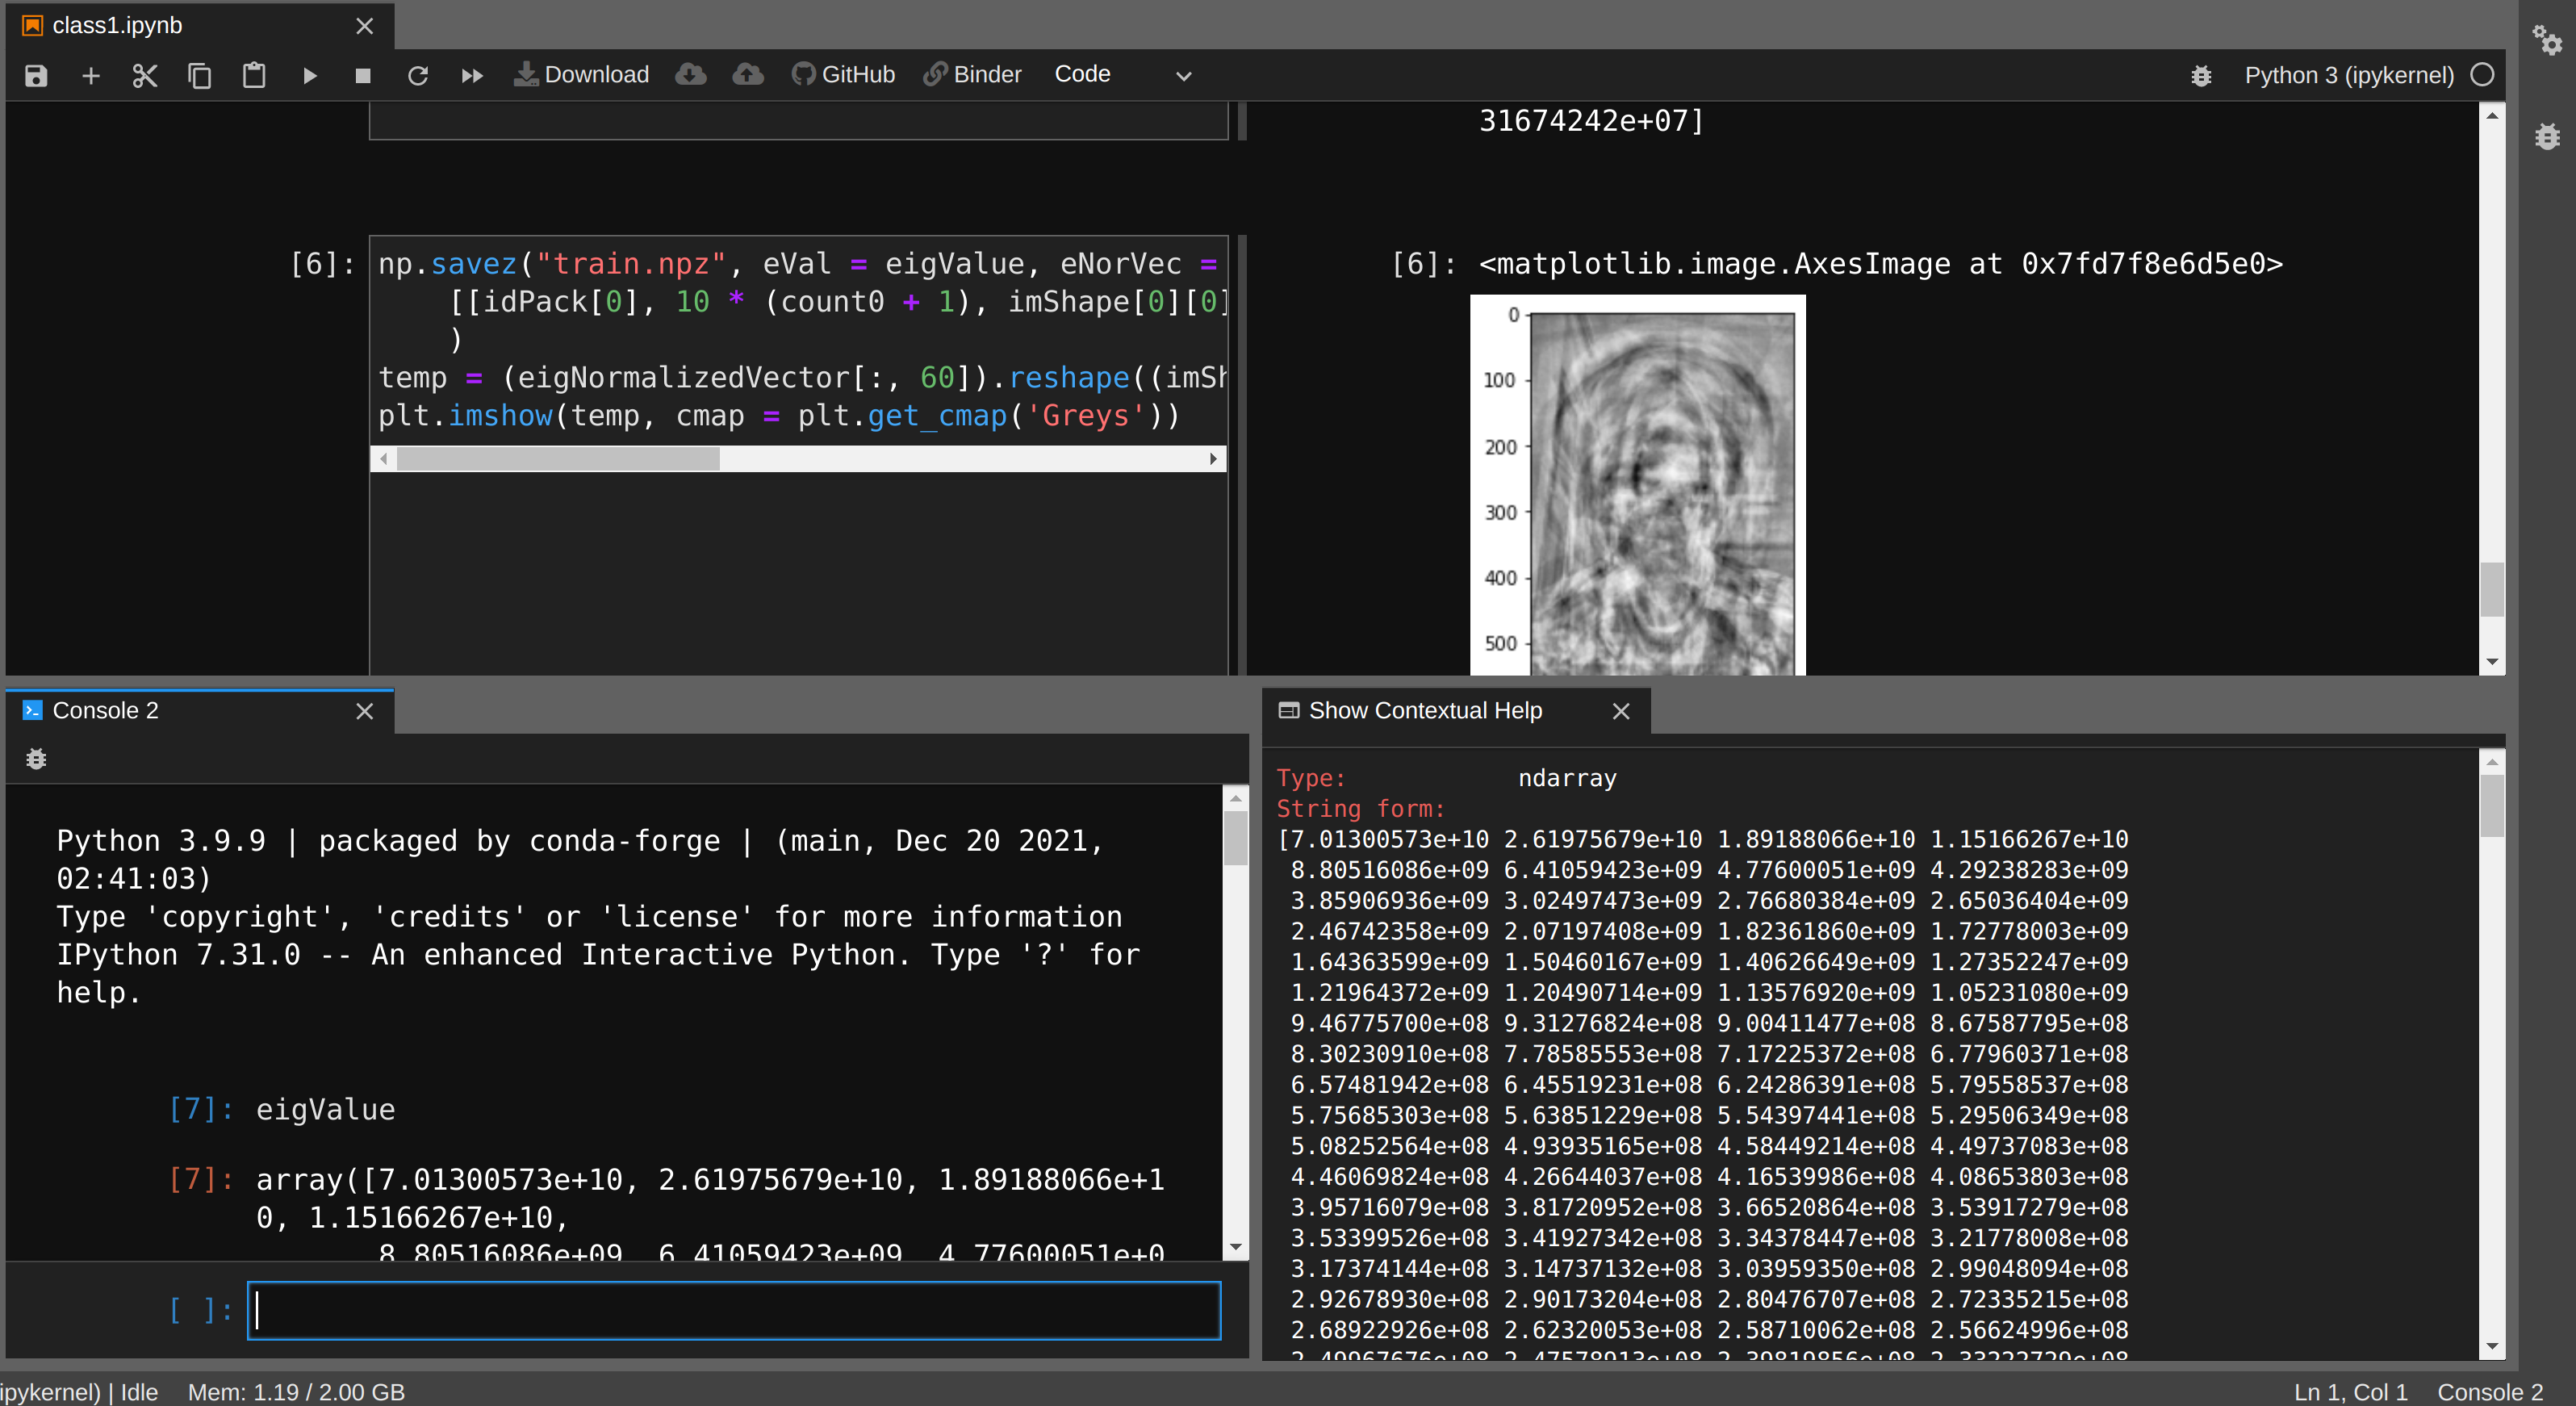
\includegraphics[width=0.9\columnwidth]{dev0.png}
    \caption{这是使用MyBinder平台,调用内核进行变量监测和查看帮助的界面。}
    \label{fig:jupyter-0}
\end{figure}
\begin{figure}[h]
    \centering
    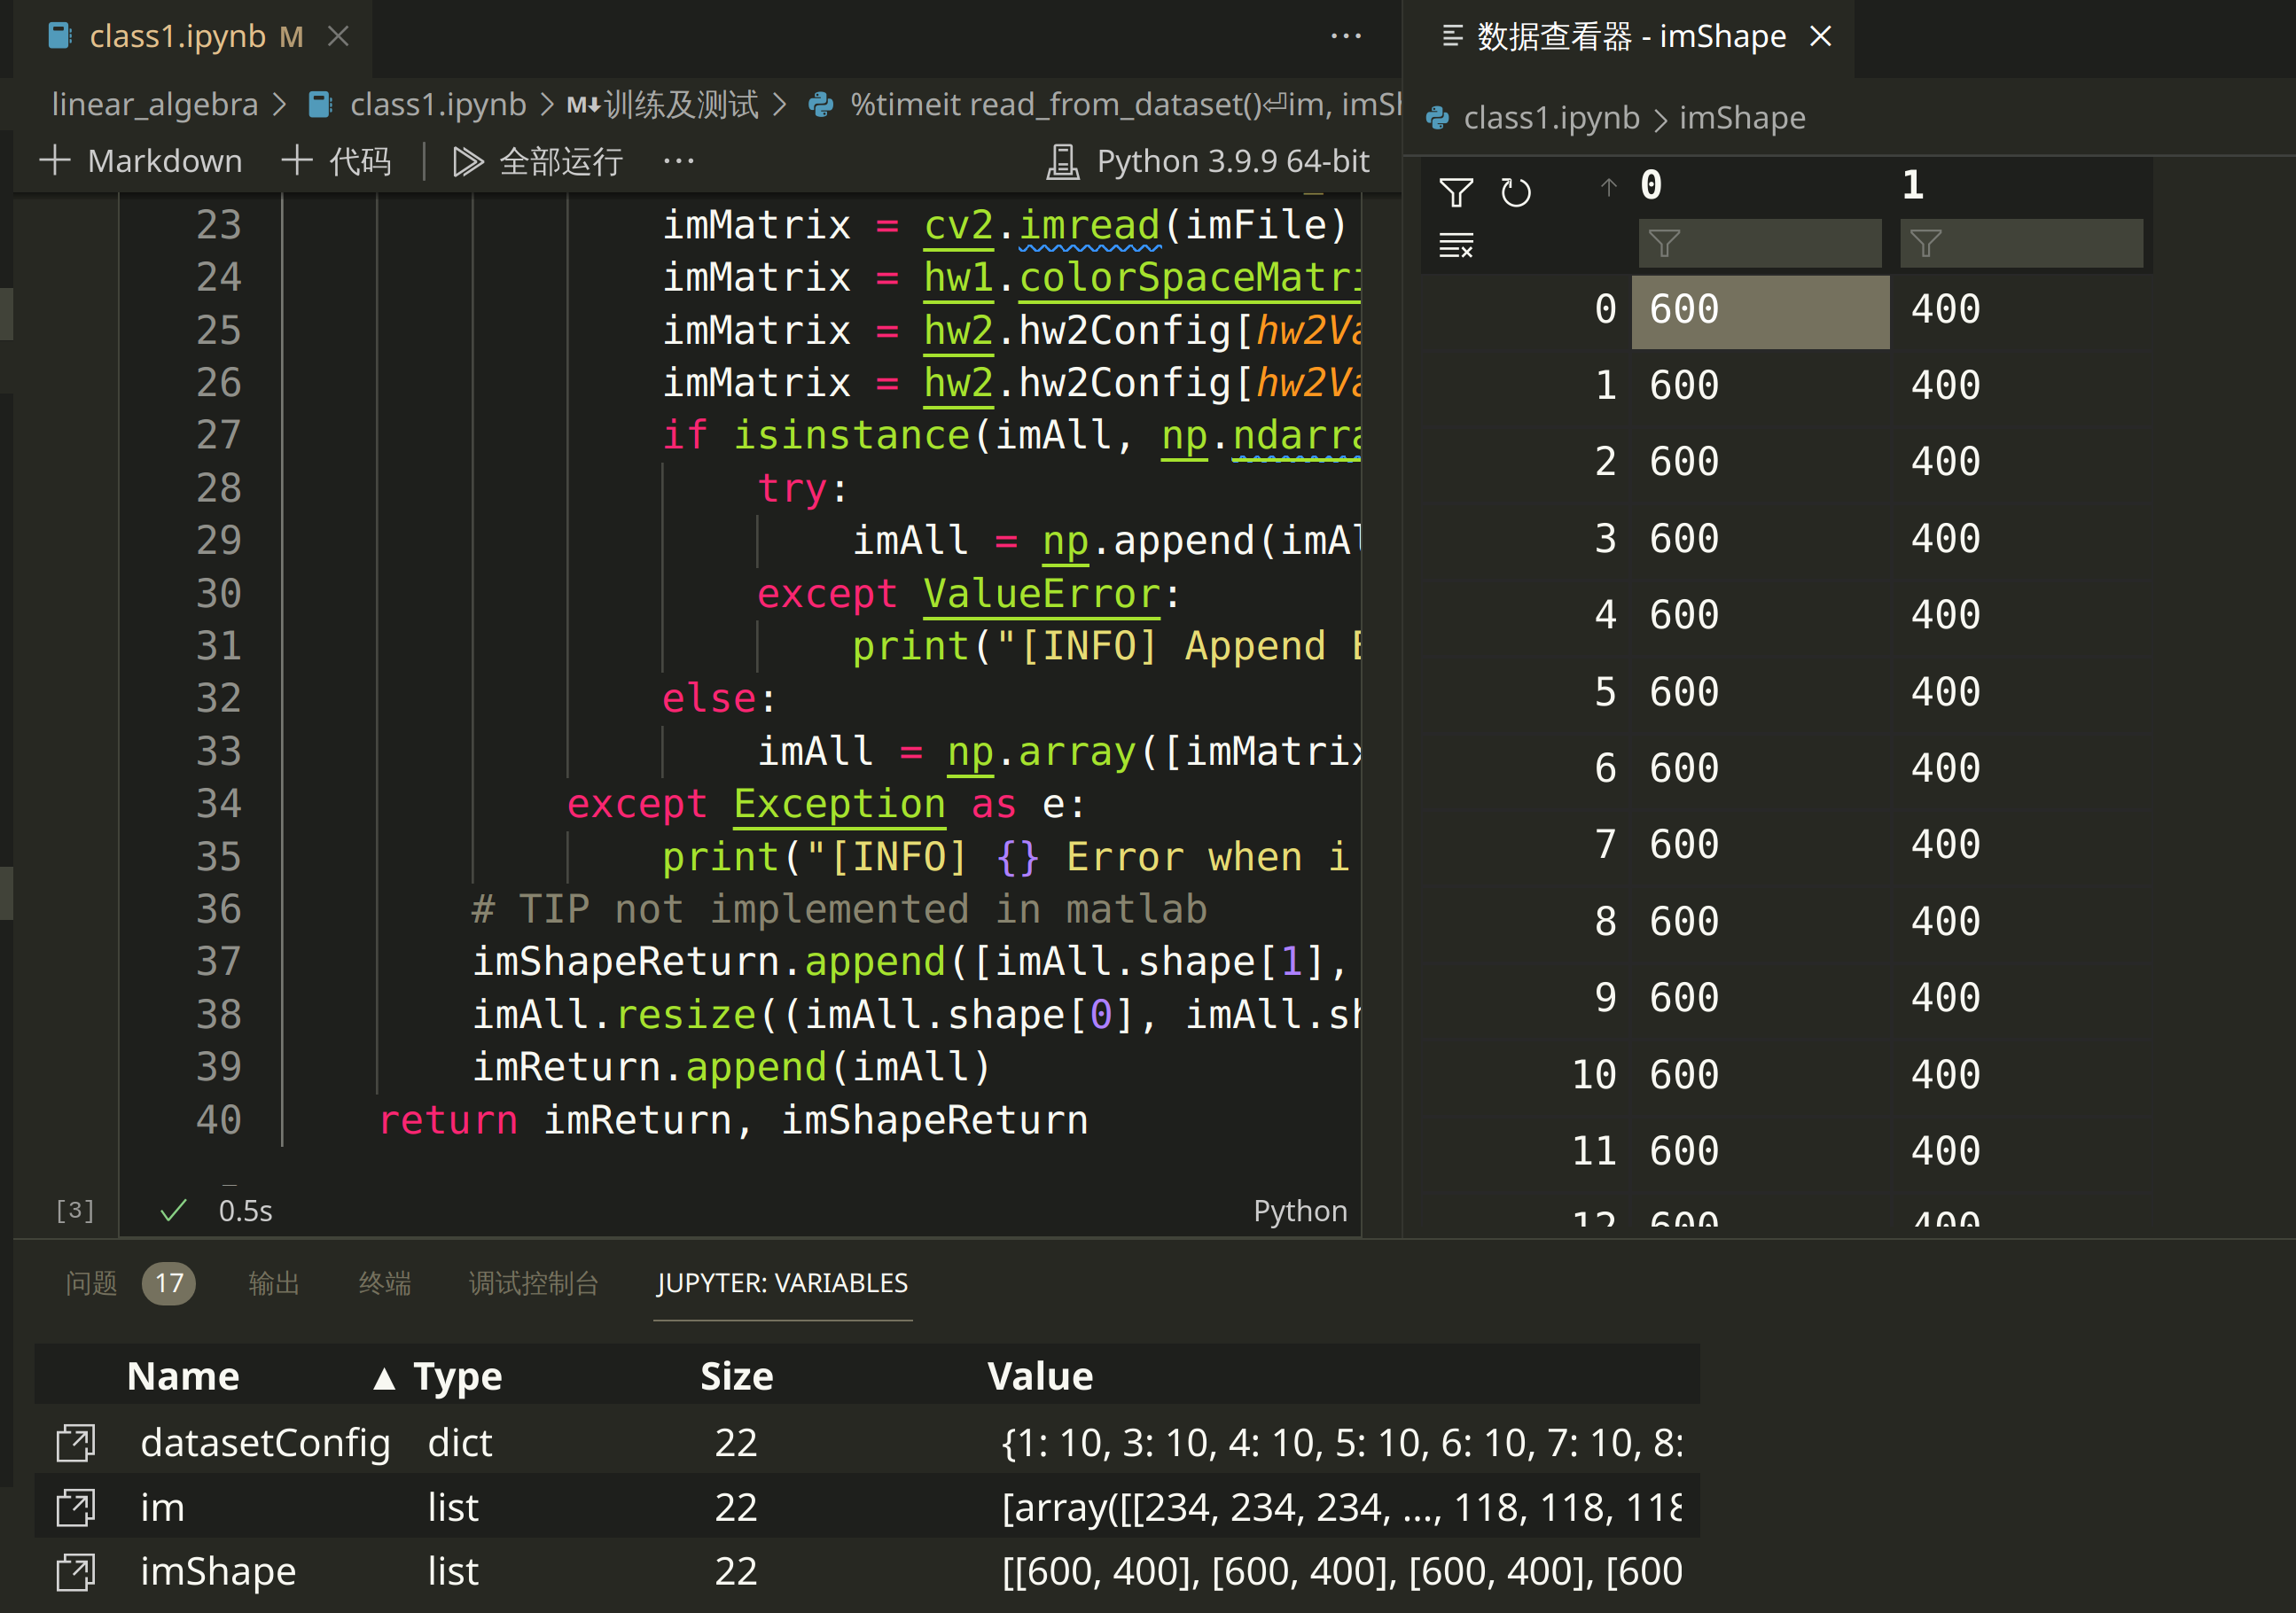
\includegraphics[width=0.9\columnwidth]{dev1.png}
    \caption{这是使用VS Code的Jupyter插件后\cite{Claudia_2021},概览数据(Data Viewer)的界面。}
    \label{fig:jupyter-1}
\end{figure}

\item \textbf{numpy}宏包是Python环境下进行矩阵运算的主流工具,与之相对应的是用于深度学习计算的\textsf{pytorch}宏包,该宏包与numpy的矩阵/张量相兼容。使用numpy宏包时,要尽可能使用自建函数代替循环,以避免动态语言执行耗时。\cite{Numpy_multi_dot}

\textbf{scipy}宏包对高阶方程运算等提供了支持。numpy.linalg依赖本包。

\textbf{scikit-learn}宏包适用于初学者对机器学习的各类工具进行直接调用。

\item \textbf{pandas}宏包完善了二维数据的可视化相关功能。\cite{GeeksForGeeks_2020}

\textbf{matplotlib}宏包完善了各类型的基本作图方法。

\textbf{opencv}宏包提供图片显示,以及跨系统的简易UI窗口创建及布局支持。

\item \textbf{实验代码预留了网络交互接口,可开发对应的GUI界面。}为了提供跨平台的支持,程序只提供静态的网站内容和数据流接口,便可达成使用手机摄像头等多设备,测试该程序的目的。这是利用Matlab难以完成的。

\item \textbf{numba}宏包基于numpy,可以通过预编译加速\verb|for loop|等费时的操作。
\end{itemize}